\let\negmedspace\undefined
\let\negthickspace\undefined
\documentclass[journal,12pt,onecolumn]{IEEEtran}
\usepackage{cite}
\usepackage{amsmath,amssymb,amsfonts,amsthm}
\usepackage{algorithmic}
\usepackage{graphicx}
\graphicspath{{./figs/}}
\usepackage{textcomp}
\usepackage{xcolor}
\usepackage{txfonts}
\usepackage{listings}
\usepackage{enumitem}
\usepackage{mathtools}
\usepackage{gensymb}
\usepackage{comment}
\usepackage{caption}
\usepackage[breaklinks=true]{hyperref}
\usepackage{tkz-euclide} 
\usepackage{listings}
\usepackage{gvv}                                        
%\def\inputGnumericTable{}                                 
%\usepackage[latin1]{inputenc}     
\usepackage{xparse}
\usepackage{color}                                            
\usepackage{array}                                            
\usepackage{longtable}                                       
\usepackage{calc}                                             
\usepackage{multirow}
\usepackage{multicol}
\usepackage{hhline}                                           
\usepackage{ifthen}                                           
\usepackage{lscape}
\usepackage{tabularx}
\usepackage{array}
\usepackage{float}
\newtheorem{theorem}{Theorem}[section]
\newtheorem{problem}{Problem}
\newtheorem{proposition}{Proposition}[section]
\newtheorem{lemma}{Lemma}[section]
\newtheorem{corollary}[theorem]{Corollary}
\newtheorem{example}{Example}[section]
\newtheorem{definition}[problem]{Definition}
\newcommand{\BEQA}{\begin{eqnarray}}
\newcommand{\EEQA}{\end{eqnarray}}
\newcommand{\define}{\stackrel{\triangle}{=}}
\theoremstyle{remark}
\newtheorem{rem}{Remark}

\setlength{\tabcolsep}{15pt}
\renewcommand{\arraystretch}{1.75}

\begin{document}

\title{GATE 2023-CE}
\author{Pratyush Panda(AI25BTECH11024)}
\maketitle

\renewcommand{\thefigure}{\theenumi}
\renewcommand{\thetable}{\theenumi}

\section*{Q. 1-Q. 25 carry one mark each.}

\begin{enumerate}
\item $\Vec{A}$  is a square matrix which is neither symmetric nor skew-symmetric and $\Vec{A^T}$ is its transpose. The sum and difference of these metrices are defined as $\Vec{S}=\Vec{A}+\Vec{A^T}$ and $\Vec{D}=\Vec{A}-\Vec{A^T}$

\hfill{\brak{\text{GATE CE 2011}}}
\begin{enumerate}
\item Both $\Vec{S}$ and $\Vec{D}$ are symmetric
\item Both $\Vec{S}$ and $\Vec{D}$ are skew-symmetric
\item $\vec{S}$ is skew-symmetric and $\vec{D}$ is symmetric
\item $\vec{S}$ is symmetric and $\vec{D}$ is skew-symmetric
\end{enumerate}

\item The square root of a number $N$ is to be obtained by applying the Newton Raphson iterations to the equation $x^2 - N = 0$. If $i$ denotes the iteration index, the correct iterative scheme will be

\hfill{\brak{\text{GATE CE 2011}}}
\begin{enumerate}
\item $x_{i+1} = \dfrac{1}{2} \left( x_i+\frac{N}{x_i}\right)$
\item $x_{i+1} = \dfrac{1}{2} \left( x_i^2+\dfrac{N}{x_i^2}\right)$
\item $x_{i+1} = \dfrac{1}{2} \left( x_i+\dfrac{N^2}{x_i}\right)$
\item $x_{i+1} = \dfrac{1}{2} \left( x_i-\dfrac{N}{x_i}\right)$
\end{enumerate}

\item There are two containers, with one containing 4 Red and 3 Green balls and the other containing 3 Blue and 4 Green balls. One ball is drawn at random from each container. The probability that one of the balls is Red and the other is Blue will be

\hfill{\brak{\text{GATE CE 2011}}}
\begin{enumerate}
\item $1/7$
\item $9/49$
\item $12/49$
\item $3/7$
\end{enumerate}

\item  For the fillet weld of size 's' shown in the adjoining figure the effective throat thickness is

\hfill{\brak{\text{GATE CE 2011}}}
\begin{figure}[H]
\centering
\includegraphics[width=0.3\columnwidth]{figs/q4.png}
\caption*{}
\label{fig:Q.4}
\end{figure}
\begin{enumerate}
\item $0.61s$
\item $0.65s$
\item $0.70s$
\item $0.75s$
\end{enumerate}

\item A $16mm$ thick plate measuring $650mm\times420mm$ is used as a base plate for an ISHB 300 column subjected to a factored axial compressive load of $2000kN$. As per IS $456-2000$, the minimum grade of concrete that should be used below the base plate for safety carrying load is

\hfill{\brak{\text{GATE CE 2011}}}
\begin{enumerate}
\item M15
\item M20
\item M30
\item M40
\end{enumerate}

\item Consider a reinforcing bar embedded in concrete. In a marine environment this bar undergoes uniform corrosion, which leads to the deposition of corrosion products on its surface and an increase in the apparent volume of the bar. This subjects the surrounding concrete to expansive pressure. As a result, corrosion induced cracks appear at the surface of concrete. Which of the following statements is TRUE?

\hfill{\brak{\text{GATE CE 2011}}}
\begin{enumerate}
\item Corrosion causes circumferential tensile stresses in concrete and the cracks will be parallel to the corroded reinforcing bar.
\item Corrosion causes radial tensile stresses in concrete and the cracks will be parallel to the corroded reinforcing bar.
\item Corrosion causes circumferential tensile stresses in concrete and the cracks will be perpendicular to the direction of the corroded reinforcing bar.
\item Corrosion causes radial tensile stresses in concrete and the cracks will be perpendicular to the direction of the corroded reinforcing bar.
\end{enumerate}

\item The results for sieve analysis carried out for three types of sand, P, Q and R, are given in the adjoining figure. If the fineness modulus values of the three sands are given as $FM_P$, $FM_Q$ and $FM_R$, it can be stated that

\hfill{\brak{\text{GATE CE 2011}}}
\begin{figure}[H]
\centering
\includegraphics[width=0.4\columnwidth]{figs/q7.png}
\caption*{}
\label{fig:Q.7}
\end{figure}
\begin{enumerate}
\item $FM_Q = \sqrt{FM_P \times FM_R}$
\item $FM_Q = 0.5 \, (FM_P + FM_R)$
\item $FM_P > FM_Q > FM_R$
\item $FM_P < FM_Q < FM_R$
\end{enumerate}

\item The cross-section of a thermo-mechanically treated (TMT) reinforcing bar has

\hfill{\brak{\text{GATE CE 2011}}}
\begin{enumerate}
\item soft ferrite-pearlite throughout.
\item hard martensite throughout.
\item a soft ferrite-pearlite core with a hard martensitic rim.
\item a hard martensitic core with a soft pearlite-bainitic rim.
\end{enumerate}

\item Consider a simply supported beam with a uniformly distributed load having a neutral axis (NA) as shown. For points P (on the neutral axis) and Q (at the bottom of the beam) the state of stress is best represented by which of the following pairs?

\hfill{\brak{\text{GATE CE 2011}}}
\begin{figure}[H]
\centering
\includegraphics[width=0.4\columnwidth]{figs/q9.png}
\caption*{}
\label{fig:Q.9}
\end{figure}
\begin{multicols}{2}
\begin{enumerate}
\item \begin{figure}[H]
\includegraphics[width=0.4\columnwidth]{figs/q9a.png}
\caption*{}
\label{fig:Q.9a}
\end{figure}
\item \begin{figure}[H]
\includegraphics[width=0.4\columnwidth]{figs/q9b.png}
\caption*{}
\label{fig:Q.9b}
\end{figure}
\item \begin{figure}[H]
\includegraphics[width=0.4\columnwidth]{figs/q9c.png}
\caption*{}
\label{fig:Q.9c}
\end{figure}
\item \begin{figure}[H]
\includegraphics[width=0.4\columnwidth]{figs/q9d.png}
\caption*{}
\label{fig:Q.9d}
\end{figure}
\end{enumerate}
\end{multicols}

\item For a saturated sand deposit, the void ratio and the specific gravity of solids are 0.70 and 2.67, respectively. The critical (upward) hydraulic gradient for the deposit would be

\hfill{\brak{\text{GATE CE 2011}}}
\begin{enumerate}
\item 0.54
\item 0.98
\item 1.02
\item 1.87
\end{enumerate}

\item Likelihood of general shear failure for an isolated footing in sand decreases with

\hfill{\brak{\text{GATE CE 2011}}}
\begin{enumerate}
\item decreasing footing depth
\item decreasing inter-granular packing of the sand
\item increasing footing width
\item decreasing soil grain compressibility
\end{enumerate}

\item For a sample of dry, cohesionless soil with friction angle $\phi$, the failure plane will be inclined to the major principal plane by an angle equal to

\hfill{\brak{\text{GATE CE 2011}}}
\begin{enumerate}
\item $\phi$
\item $45^\circ$
\item $45^\circ - \phi/2$
\item $45^\circ + \phi/2$
\end{enumerate}

\item Two geometrically identical isolated footings, $X$ (linear elastic) and $Y$ (rigid), are loaded identically (shown alongside). The soil reactions will

\hfill{\brak{\text{GATE CE 2011}}}
\begin{figure}[H]
\centering
\includegraphics[width=0.4\columnwidth]{figs/q13.png}
\caption*{}
\label{fig:Q.13}
\end{figure}
\begin{enumerate}
\item be uniformly distributed for $Y$ but not for $X$
\item be uniformly distributed for $X$ but not for $Y$
\item be uniformly distributed for both $X$ and $Y$
\item not be uniformly distributed for both $X$ and $Y$
\end{enumerate}

\item A soil is composed of solid spherical grains of identical specific gravity and diameter between 0.075 mm and 0.0075 mm. If the terminal velocity of the largest particle falling through water without flocculation is 0.5 mm/s, that for the smallest particle would be

\hfill{\brak{\text{GATE CE 2011}}}
\begin{enumerate}
\item 0.005 mm/s
\item 0.05 mm/s
\item 5 mm/s
\item 50 mm/s
\end{enumerate}

\item A watershed got transformed from rural to urban over a period of time. The effect of urbanization on storm runoff hydrograph from the watershed is to

\hfill{\brak{\text{GATE CE 2011}}}
\begin{enumerate}
\item decrease the volume of runoff
\item increase the time to peak discharge
\item decrease the time base
\item decrease the peak discharge
\end{enumerate}

\item For a given discharge, the critical flow depth in an open channel depends on

\hfill{\brak{\text{GATE CE 2011}}}
\begin{enumerate}
\item channel geometry only
\item channel geometry and bed slope
\item channel geometry, bed slope and roughness
\item channel geometry, bed slope, roughness and Reynolds number
\end{enumerate}

\item For a body completely submerged in a fluid, the centre of gravity (G) and centre of buoyancy (O) are known. The body is considered to be in stable equilibrium if

\hfill{\brak{\text{GATE CE 2011}}}
\begin{enumerate}
\item O does not coincide with the centre of mass of the displaced fluid
\item G coincides with the centre of mass of the displaced fluid
\item O lies below G
\item O lies above G
\end{enumerate}

\item The flow in a horizontal, frictionless rectangular open channel is supercritical. A smooth hump is built on the channel floor. As the height of hump is increased, choked condition is attained. With further increase in the height of the hump, the water surface will

\hfill{\brak{\text{GATE CE 2011}}}
\begin{enumerate}
\item rise at a section upstream of the hump
\item drop at a section upstream of the hump
\item drop at the hump
\item rise at the hump
\end{enumerate}

\item Consider the following unit processes commonly used in water treatment; rapid mixing (RM), flocculation (F), primary sedimentation (PS), secondary sedimentation (SS), chlorination (C) and rapid sand filtration (RSF). The order of these unit processes (first to last) in a conventional water treatment plant is

\hfill{\brak{\text{GATE CE 2011}}}
\begin{enumerate}
\item PS $\rightarrow$ RSF $\rightarrow$ F $\rightarrow$ RM $\rightarrow$ SS $\rightarrow$ C
\item PS $\rightarrow$ F $\rightarrow$ RM $\rightarrow$ RSF $\rightarrow$ SS $\rightarrow$ C
\item PS $\rightarrow$ F $\rightarrow$ SS $\rightarrow$ RSF $\rightarrow$ RM $\rightarrow$ C
\item PS $\rightarrow$ RM $\rightarrow$ F $\rightarrow$ SS $\rightarrow$ RSF $\rightarrow$ C
\end{enumerate}

\item Anaerobically treated effluent has MPN of total coliforms as $10^6$/100 mL. After chlorination, the MPN value declines to $10^2$/100 mL. The percent removal (\%R) and log removal (log R) of total coliform MPN is

\hfill{\brak{\text{GATE CE 2011}}}
\begin{enumerate}
\item \%R = 99.90; log R = 4
\item \%R = 99.90; log R = 2
\item \%R = 99.99; log R = 4
\item \%R = 99.99; log R = 2
\end{enumerate}

\item Consider four common air pollutants found in urban environments, NO, SO$_2$, Soot and O$_3$. Among these which one is the secondary air pollutant?

\hfill{\brak{\text{GATE CE 2011}}}
\begin{enumerate}
\item O$_3$
\item NO
\item SO$_2$
\item Soot
\end{enumerate}

\item The probability that $k$ number of vehicles arrive (i.e. cross a predefined line) in time $t$ is given as $(\lambda t)^k e^{-\lambda t}/k!$, where $\lambda$ is the average vehicle arrival rate. What is the probability that the time headway is greater than or equal to time $t_1$?

\hfill{\brak{\text{GATE CE 2011}}}
\begin{enumerate}
\item $\lambda e^{\lambda t_1}$
\item $\lambda e^{-\lambda t_1}$
\item $e^{\lambda t_1}$
\item $e^{-\lambda t_1}$
\end{enumerate}

\item A vehicle negotiates a transition curve with uniform speed $v$. If the radius of the horizontal curve and the allowable jerk are $R$ and $J$, respectively, the minimum length of the transition curve is

\hfill{\brak{\text{GATE CE 2011}}}
\begin{enumerate}
\item $R^3/(vJ)$
\item $J^3/(Rv)$
\item $v^2 R/J$
\item $v^3/(RJ)$
\end{enumerate}

\item In Marshall testing of bituminous mixes, as the bitumen content increases the flow value

\hfill{\brak{\text{GATE CE 2011}}}
\begin{enumerate}
\item remains constant
\item decreases first and then increases
\item increases monotonically
\item increases first and then decreases
\end{enumerate}

\item Curvature correction for staff reading in a differential leveling survey is

\hfill{\brak{\text{GATE CE 2011}}}
\begin{enumerate}
\item always additive
\item always zero
\item always subtractive
\item depends on latitude
\end{enumerate}

\section*{Q. 26 to Q. 55 carry two marks each.}

\item For an analytic function, $f(x+iy) = u(x, y) + iv(x, y)$, $u$ is given by $u = 3x^2 - 3y^2$. The expression for $v$, considering $K$ to be a constant is

\hfill{\brak{\text{GATE CE 2011}}}
\begin{enumerate}
\item $3y^2 - 3x^2 + K$
\item $6x - 6y + K$
\item $6y - 6x + K$
\item $6xy + K$
\end{enumerate}

\item What should be the value of $\lambda$ such that the function defined below is continuous at $x = \pi/2?$

\hfill{\brak{\text{GATE CE 2011}}}
$f(x) = 
\begin{cases}
\dfrac{\lambda \cos x}{\frac{\pi}{2} - x} & \text{if } x \neq \pi/2 \\
1 & \text{if } x = \pi/2
\end{cases}$
\begin{enumerate}[label=(\Alph*)]
\item $0$
\item $2/\pi$
\item $1$
\item $\pi/2$
\end{enumerate}

\item What is the value of the definite integral, $\displaystyle\int_0^a \frac{\sqrt{x}}{\sqrt{x} + \sqrt{a-x}}\ dx$?

\hfill{\brak{\text{GATE CE 2011}}}
\begin{enumerate}
\item $0$
\item $a/2$
\item $a$
\item $2a$
\end{enumerate}

\item If $\vec{a}$ and $\vec{b}$ are two arbitrary vectors with magnitudes $a$ and $b$, respectively, $|\vec{a} \times \vec{b}|^2$ will be equal to

\hfill{\brak{\text{GATE CE 2011}}}
\begin{enumerate}
\item $a^2 b^2 - \left(\vec{a} \cdot \vec{b}\right)^2$
\item $ab - \vec{a} \cdot \vec{b}$
\item $a^2 b^2 + \left(\vec{a} \cdot \vec{b}\right)^2$
\item $ab + \vec{a} \cdot \vec{b}$
\end{enumerate}

\item The solution of the differential equation $\dfrac{dy}{dx} + \dfrac{y}{x} = x$, with the condition that $y = 1$ at $x = 1$, is

\hfill{\brak{\text{GATE CE 2011}}}
\begin{enumerate}
\item $y = \dfrac{2}{3x^2} + \dfrac{x}{3}$
\item $y = \dfrac{x}{2} + \dfrac{1}{2x}$
\item $y = \dfrac{2}{3} + \dfrac{x}{3}$
\item $y = \dfrac{2}{3x} + \dfrac{x^2}{3}$
\end{enumerate}

\item The value of $W$ that results in the collapse of the beam shown in the adjoining figure and having a plastic moment capacity of $M_p$ is

\hfill{\brak{\text{GATE CE 2011}}}
\begin{figure}[H]
\centering
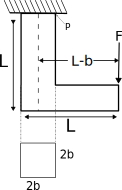
\includegraphics[width=0.4\columnwidth]{figs/q31.png}
\caption*{}
\label{fig:Q.31}
\end{figure}
\begin{enumerate}
\item $(4/21)\, M_p$
\item $(3/10)\, M_p$
\item $(7/21)\, M_p$
\item $(13/21)\, M_p$
\end{enumerate}

\item For the cantilever bracket, PQRS, loaded as shown in the adjoining figure $\brak{\text{PQ = RS = L, and QR = 2L}}$, which of the following statements is FALSE?

\hfill{\brak{\text{GATE CE 2011}}}
\begin{figure}[H]
\centering
\includegraphics[width=0.4\columnwidth]{figs/q32.png}
\caption*{}
\label{fig:Q.32}
\end{figure}
\begin{enumerate}
\item The portion RS has a constant twisting moment with a value of 2WL.
\item The portion QR has a varying twisting moment with a maximum value of WL.
\item The portion PQ has a varying bending moment with a maximum value of WL.
\item The portion PQ has no twisting moment.
\end{enumerate}

\item Consider a bar of diameter $D$ embedded in a large concrete block as shown in the adjoining figure, with a pull out force $P$ being applied. Let $\sigma_b$ and $\sigma_t$ be the bond strength $\brak{\text{between the bar and concrete}}$ and the tensile strength of the bar, respectively. If the block is held in position and it is assumed that the material of the block does not fail, which of the following options represents the maximum value of $P$?

\hfill{\brak{\text{GATE CE 2011}}}
\begin{figure}[H]
\centering
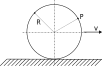
\includegraphics[width=0.4\columnwidth]{figs/q33.png}
\caption*{}
\label{fig:Q.33}
\end{figure}
\begin{enumerate}
\item Maximum of $\left(\dfrac{\pi}{4} D^2 \sigma_t\right)$ and $(\pi D L \sigma_b)$
\item Maximum of $\left(\dfrac{\pi}{4} D^2 \sigma_b\right)$ and $(\pi D L \sigma_t)$
\item Minimum of $\left(\dfrac{\pi}{4} D^2 \sigma_t\right)$ and $(\pi D L \sigma_b)$
\item Minimum of $\left(\dfrac{\pi}{4} D^2 \sigma_b\right)$ and $(\pi D L \sigma_t)$
\end{enumerate}

\item Consider two RCC beams, P and Q, each having the section $400 mm \times 750 mm$ $\brak{\text{effective depth, }d = 750 mm}$ made with concrete having a $\tau_{\mathrm{v,max}} = 2.1$ N/mm$^2$. For the reinforcement provided and the grade of concrete used, it may be assumed that the $\tau_c = 0.75$ N/mm$^2$. The design shear in beam P is $400 kN$ and in beam Q is $750 kN$. Considering the provisions of IS 456 – 2000, which of the following statements is TRUE?

\hfill{\brak{\text{GATE CE 2011}}}
\begin{enumerate}
\item Shear reinforcement should be designed for $175 kN$ for beam P and the section for beam Q should be revised.
\item Nominal shear reinforcement is required for beam P and the shear reinforcement should be designed for $120 kN$ for beam Q.
\item The section for beam P should be designed for $175 kN$ for beam P and the shear reinforcement should be designed for $525 kN$ for beam Q.
\item The sections for both beams P and Q need to be revised.
\end{enumerate}

\item The adjoining figure shows a schematic representation of a steel plate girder to be used as a simply supported beam with an upward concentrated load. For stiffeners, PQ $\brak{\text{running along the beam axis}}$ and RS $\brak{\text{running between the top and bottom flanges}}$ which of the following pairs of statements will be TRUE?

\hfill{\brak{\text{GATE CE 2011}}}
\begin{figure}[H]
\centering
\includegraphics[width=0.4\columnwidth]{figs/q35.png}
\caption*{}
\label{fig:Q.35}
\end{figure}
\begin{enumerate}
\item (i) RS should be provided under the concentrated load only.\\
      (ii) PQ should be placed in the tension side of the flange.
\item (i) RS helps to prevent local buckling of the web.\\
      (ii) PQ should be placed in the compression side of the flange.
\item (i) RS should be provided at supports.\\
      (ii) PQ should be placed along the neutral axis.
\item (i) RS should be provided away from points of action of concentrated loads.\\
      (ii) PQ should be provided on the compression side of the flange.
\end{enumerate}

\item A singly under-reamed, $8m$ long, RCC pile $\brak{\text{shown in the adjoining figure}}$ weighting $20 kN$ with $350 mm$ shaft diameter and $750 mm$ under-ream diameter is installed within stiff, saturated silty clay $\brak{\text{undrained shear strength is 50 kPa, adhesion factor is 0.3, and the applicable bearing capacity factor is 9}}$ to counteract the impact of soil swelling on a structure constructed above. Neglecting suction and the contribution of the under-ream to my adhesive shaft capacity, what would be the estimated ultimate tensile capacity $\brak{\text{rounded off to the nearest integer value of kN}}$ of the pile?

\hfill{\brak{\text{GATE CE 2011}}}
\begin{figure}[H]
\centering
\includegraphics[width=0.25\columnwidth]{figs/q36.png}
\caption*{}
\label{fig:Q.36}
\end{figure}
\begin{enumerate}
\item $132 kN$
\item $156 kN$
\item $287 kN$
\item $301 kN$
\end{enumerate}

\item Identical surcharges are placed at ground surface at sites $X$ and $Y$, with soil conditions shown alongside and water table at ground surface. The silty clay layers at $X$ and $Y$ are identical. The thin sand layer at $Y$ is continuous and free-draining with a very large discharge capacity. If primary consolidation at $X$ is estimated to complete in 36 months, what would be the average corresponding time for completion of primary consolidation at $Y$?

\hfill{\brak{\text{GATE CE 2011}}}
\begin{figure}[H]
\centering
\includegraphics[width=0.3\columnwidth]{figs/q37.png}
\caption*{}
\label{fig:Q.37}
\end{figure}
\begin{enumerate}
\item 2.25 months
\item 4.5 months
\item 9 months
\item 36 months
\end{enumerate}

\item A field vane shear testing instrument $\brak{\text{shown alongside}}$ was inserted completely into a deposit of soft, saturated silty clay with the vane rod vertical such that the top of the blades were $500mm$ below the ground surface. Upon application of a rapidly increasing torque about the vane rod, the soil was found to fail when the torque reached $4.6Nm$. Assuming mobilization of undrained shear strength on all failure surfaces to be uniform and the resistance mobilized on the surface of the vane rod to be negligible, what would be the peak undrained shear strength $\brak{\text{rounded off to the nearest integer value of kPa}}$ of the soil?

\hfill{\brak{\text{GATE CE 2011}}}
\begin{figure}[H]
\centering
\includegraphics[width=0.25\columnwidth]{figs/q38.png}
\caption*{}
\label{fig:Q.38}
\end{figure}
\begin{enumerate}
\item $5 kPa$
\item $10 kPa$
\item $15 kPa$
\item $20 kPa$
\end{enumerate}

\item A single pipe of length $1500m$ and diameter $60cm$ connects two reservoirs having a difference of $20m$ in their water levels. The pipe is to be replaced by two pipes of the same length and equal diameter $d$ to convey $25\%$ more discharge under the same head loss. If the friction factor is assumed to be the same for all the pipes, the value of $d$ is approximately equal to which of the following options?

\hfill{\brak{\text{GATE CE 2011}}}
\begin{enumerate}
\item $37.5cm$
\item $40.0cm$
\item $45.0cm$
\item $50.0cm$
\end{enumerate}

\item A spillway discharges flood flow at a rate of $9m^3/s$ per metre width. If the depth of flow on the horizontal apron at the toe of the spillway is $46cm$, the tail water depth needed to form a hydraulic jump is approximately given by which of the following options?

\hfill{\brak{\text{GATE CE 2011}}}
\begin{enumerate}
\item $2.54m$
\item $4.90m$
\item $5.77m$
\item $6.23m$
\end{enumerate}

\item In an aquifer extending over 150 hectare, the water table was $20m$ below ground level. Over a period of time the water table dropped to $23m$ below the ground level. If the porosity of aquifer is 0.40 and the specific retention is 0.15, what is the change in ground water storage of the aquifer?

\hfill{\brak{\text{GATE CE 2011}}}
\begin{enumerate}
\item $67.5 \,ha-m$
\item $112.5 \,ha-m$
\item $180.0 \, ha-m$
\item $450.0 \,ha-m$
\end{enumerate}

\item Total suspended particulate matter (TSP) concentration in ambient air is to be measured using a high volume sampler. The filter used for this purpose had an initial dry weight of $9.787~g$. The filter was mounted in the sampler and the initial air flow rate through the filter was set at $1.5~m^3/min$. Sampling continued for 24 hours. The airflow after 24 hours was measured to be $1.4~m^3/min$. The dry weight of the filter paper after 24 hours sampling was $10.283~g$. Assuming a linear decline in the air flow rate during sampling, what is the 24 hour average TSP concentration in ambient air?

\hfill{\brak{\text{GATE CE 2011}}}
\begin{enumerate}
\item $59.2~\mu g/m^3$
\item $118.6~\mu g/m^3$
\item $237.5~\mu g/m^3$
\item $574.4~\mu g/m^3$
\end{enumerate}

\item Chlorine gas $\brak{8~mg/L~as~Cl_2}$ was added to a drinking water sample. If the free chlorine residual and pH was measured to be $2~mg/L~\brak{as~Cl_2}$ and 7.5, respectively, what is the concentration of residual $OCl^-$ ions in the water? Assume that the chlorine gas added to the water is completely converted to $HOCl$ and $OCl^-$. Atomic Weight of Cl: 35.5

Given: $\text{OCl}^- + \text{H}^+ \xleftrightarrow{\text{K}} \text{HOCl}$,\quad $K = 10^{-7.5}$

\hfill{\brak{\text{GATE CE 2011}}}
\begin{enumerate}
\item $1.408 \times 10^{-5}$ moles/L
\item $2.817 \times 10^{-5}$ moles/L
\item $5.634 \times 10^{-5}$ moles/L
\item $1.127 \times 10^{-4}$ moles/L
\end{enumerate}

\item If the jam density is given as $k_j$ and the free flow speed is given as $u_f$, the maximum flow for a linear traffic speed-density model is given by which of the following options?

\hfill{\brak{\text{GATE CE 2011}}}
\begin{enumerate}
\item $\dfrac{1}{4} k_j u_f$
\item $\dfrac{1}{3} k_j u_f$
\item $\dfrac{3}{5} k_j u_f$
\item $\dfrac{2}{3} k_j u_f$
\end{enumerate}

\item If $v$ is the initial speed of a vehicle, $g$ is the gravitational acceleration, $G$ is the upward longitudinal slope of the road and $f_r$ is the coefficient of rolling friction during braking, the braking distance $\brak{\text{measured horizontally}}$ for the vehicle to stop is

\hfill{\brak{\text{GATE CE 2011}}}
\begin{enumerate}
\item $\dfrac{v^2}{g \left( G + f_r \right)}$
\item $\dfrac{v^2}{2g \left( G + f_r \right)}$
\item $\dfrac{vg}{\left( G + f_r \right)}$
\item $\dfrac{vf_r}{\left( G + g \right)}$
\end{enumerate}

\item The cumulative arrival and departure curve of one cycle of an approach lane of a signalized intersection is shown in the adjoining figure. The cycle time is $50 s$ and the effective red time is $30 s$ and the effective green time is $20 s$. What is the average delay?

\hfill{\brak{\text{GATE CE 2011}}}
\begin{figure}[H]
\centering
\includegraphics[width=0.3\columnwidth]{figs/q46.png}
\caption*{}
\label{fig:Q.46}
\end{figure}
\begin{enumerate}
\item 15 s
\item 25 s
\item 35 s
\item 45 s
\end{enumerate}

\item The observations from a closed loop traverse around an obstacle are

\begin{table}[H]
\centering
\begin{tabular}{|c|c|c|c|}
\hline
Segment & Observation from station & Length (m) & Azimuth (clockwise from magnetic north) \\
\hline
PQ & P & Missing & $33.7500^\circ$ \\
\hline
QR & Q & $300.000$ & $86.3847^\circ$ \\
\hline
RS & R & $354.524$ & $169.3819^\circ$ \\
\hline
ST & S & $450.000$ & $243.9003^\circ$ \\
\hline
TP & T & $268.000$ & $317.5000^\circ$ \\
\hline
\end{tabular}
\caption*{}
\label{tab:Q.47}
\end{table}
What is the value of the missing measurement $\brak{\text{rounded off to nearest }10mm}$

\hfill{\brak{\text{GATE CE 2011}}}
\begin{enumerate}
\item $ 396.86 m$
\item $396.79 m$
\item $396.05 m$
\item $396.94 m$
\end{enumerate}

\subsection*{Common Data Questions}
\textbf{Common Data for Questions 48 and 49:}

A sand layer found at sea floor under $20 m$ water depth is characterized with relative density = 40 \%, maximum void ratio = 1.0, minimum void ratio = 0.5, and specific gravity of soil solids = 2.67. Assume the specific gravity of sea water to be 1.03 and the unit weight of fresh water to be $9.81 kN/m³$.

\item What would be the effective stress $\brak{\text{rounded off to the nearest integer value of kPa}}$ at 30 m depth into the sand layer?

\hfill{\brak{\text{GATE CE 2011}}}
\begin{enumerate}
\item $77kPa$
\item $273kPa$
\item $268kPa$
\item $281kPa$
\end{enumerate}

\item What would be the change in the effective stress $\brak{\text{rounded off to the nearest integer value of kPa}}$ at $30 m$ depth into the sand layer if the sea water level permanently rises by $2 m$?

\hfill{\brak{\text{GATE CE 2011}}}
\begin{enumerate}
\item $19kPa$
\item $0kPa$
\item $21kPa$
\item $22kPa$
\end{enumerate}

\textbf{Common Data for Questions 50 and 51:}

The ordinates of a 2-h unit hydrograph at 1 hour intervals starting from time t = 0, are 0, 3, 8, 6, 3, 2 and 0 $m^3/s$. Use trapezoidal rule for numerical integration, if required.

\item What is the catchment area represented by the unit hydrograph?

\hfill{\brak{\text{GATE CE 2011}}}
\begin{enumerate}
\item $1.00km^2$
\item $2.00km^2$
\item $7.92km^2$
\item $8.64km^2$
\end{enumerate}

\item A storm of $6.6 cm$ occurs uniformly over the catchment in 3 hours. If Q-index is equal to $2 mm/h$ and base flow is $5 m^3/s$, what is the peak flow due to the storm?

\hfill{\brak{\text{GATE CE 2011}}}
\begin{enumerate}
\item $41.0 m^3/s$
\item $43.4 m^3/s$
\item $53.0 m^3/s$
\item $56.2 m^3/s$
\end{enumerate}

\subsection*{Linked Answer Questions}
\textbf{Statement for Linked Answer Questions 52 and 53:}

A rigid beam is hinged at one end and supported on linear elastic springs $\brak{\text{both having a stiffness of 'k'}}$ at points '1' and '2', and an inclined load acts at '2', as shown.

\begin{figure}[H]
\centering
\includegraphics[width=0.4\columnwidth]{figs/q52,53.png}
\caption*{}
\label{fig:Q.52,53}
\end{figure}
\item Which of the following options represents the deflections $\delta_1$ and $\delta_2$ at points '1' and '2'?

\hfill{\brak{\text{GATE CE 2011}}}
\begin{enumerate}
\item $\delta_1 = \dfrac{2}{5}\left(\dfrac{2P}{k}\right)$ and $\delta_2 = \dfrac{4}{5}\left(\dfrac{2P}{k}\right)$
\item $\delta_1 = \dfrac{2}{5}\left(\dfrac{P}{k}\right)$ and $\delta_2 = \dfrac{4}{5}\left(\dfrac{P}{k}\right)$
\item $\delta_1 = \dfrac{2}{5}\left(\dfrac{P}{\sqrt{2}k}\right)$ and $\delta_2 = \dfrac{4}{5}\left(\dfrac{P}{\sqrt{2}k}\right)$
\item $\delta_1 = \dfrac{2}{5}\left(\dfrac{\sqrt{2}P}{k}\right)$ and $\delta_2 = \dfrac{4}{5}\left(\dfrac{\sqrt{2}P}{k}\right)$
\end{enumerate}

\item If the load P equals $100 kN$, which of the following options represents forces $R_1$ and $R_2$ in the springs at points '1' and '2'?

\hfill{\brak{\text{GATE CE 2011}}}
\begin{enumerate}
\item $R_1 = 20 kN$ and $R_2 = 40 kN$
\item $R_1 = 50 kN$ and $R_2 = 50 kN$
\item $R_1 = 30 kN$ and $R_2 = 60 kN$
\item $R_1 = 40 kN$ and $R_2 = 80 kN$
\end{enumerate}

\textbf{Statement for Linked Answer Questions 54 and 55:}

The sludge from the aeration tank of the activated sludge process (ASP) has solids content $\brak{\text{by weight}}$ of $2\%$. This sludge is put in a sludge thickener, where sludge volume is reduced to half. Assume that the amount of solids in the supernatant from the thickener is negligible, the specific gravity of sludge solids is 2.2 and the density of water is $1000 kg/m^3$.

\item What is the density of the sludge removed from the aeration tank?

\hfill{\brak{\text{GATE CE 2011}}}
\begin{enumerate}
\item $990 kg/m^3$
\item $1000 kg/m^3$
\item $1011 kg/m^3$
\item $1022 kg/m^3$
\end{enumerate}

\item What is the solids content $\brak{\text{by weight}}$ of the thickened sludge?

\hfill{\brak{\text{GATE CE 2011}}}
\begin{enumerate}
\item $3.96\%$
\item $4.00\%$
\item $4.04\%$
\item $4.10\%$
\end{enumerate}

\section*{General Aptitude (GA) Questions}
\section*{Q. 56- Q. 60 carry one mark each.}

\item If $\log (P) = \frac{1}{2}\log (Q) = \frac{1}{3}\log (R)$, then which of the following options is TRUE?

\hfill{\brak{\text{GATE CE 2011}}}
\begin{enumerate}
\item $P^2 = Q^3 R^2$
\item $Q^2 = PR$
\item $Q^2 = R^3 P$
\item $R = P^2 Q^2$
\end{enumerate}

\item Which of the following options is the closest in meaning to the word below: \\
\textbf{Inexplicable}

\hfill{\brak{\text{GATE CE 2011}}}
\begin{enumerate}
\item Incomprehensible
\item Indelible
\item Inextricable
\item Infallible
\end{enumerate}

\item Choose the word from the options given below that is most nearly opposite in meaning to the given word: \\
\textbf{Amalgamate}

\hfill{\brak{\text{GATE CE 2011}}}
\begin{enumerate}
\item merge
\item split
\item collect
\item separate
\end{enumerate}

\item Choose the most appropriate word from the options given below to complete the following sentence. \\
\textbf{If you are trying to make a strong impression on your audience, you cannot do so by being understated, tentative or \rule{3cm}{0.15mm}.}

\hfill{\brak{\text{GATE CE 2011}}}
\begin{enumerate}
\item hyperbolic
\item restrained
\item argumentative
\item indifferent
\end{enumerate}

\item Choose the most appropriate word(s) from the options given below to complete the following sentence. \\
\textbf{I contemplated \rule{3cm}{0.15mm} Singapore for my vacation but decided against it.}

\hfill{\brak{\text{GATE CE 2011}}}
\begin{enumerate}
\item to visit
\item having to visit
\item visiting
\item for a visit
\end{enumerate}

\section*{Q. 61 to Q. 65 carry two marks each.}
\item P, Q, R and S are four types of dangerous microbes recently found in a human habitat. The area of each circle with its diameter printed in brackets represents the growth of a single microbe surviving human immunity system within 24 hours of entering the body. The danger to human beings varies proportionally with the toxicity, potency and growth attributed to a microbe shown in the figure below:

\begin{figure}[H]
\centering
\includegraphics[width=0.4\columnwidth]{figs/q61.png}
\caption*{}
\label{fig:Q.61}
\end{figure}

A pharmaceutical company is contemplating the development of a vaccine against the most dangerous microbe. Which microbe should the company target in its first attempt?

\hfill{\brak{\text{GATE CE 2011}}}
\begin{enumerate}
\item P
\item Q
\item R
\item S
\end{enumerate}

\item \textbf{Few school curricula include a unit on how to deal with bereavement and grief, and yet all students at some point in their lives suffer from losses through death and parting.}

Based on the above passage which topic would not be included in a unit on bereavement?

\hfill{\brak{\text{GATE CE 2011}}}
\begin{enumerate}
\item how to write a letter of condolence
\item what emotional stages are passed through in the healing process
\item what the leading causes of death are
\item how to give support to a grieving friend
\end{enumerate}

\item A container originally contains 10 litres of pure spirit. From this container 1 litre of spirit is replaced with 1 litre of water. Subsequently, 1 litre of the mixture is again replaced with 1 litre of water and this process is repeated one more time. How much spirit is now left in the container?

\hfill{\brak{\text{GATE CE 2011}}}
\begin{enumerate}
\item 7.58 litres
\item 7.84 litres
\item 7 litres
\item 7.29 litres
\end{enumerate}

\item A transporter receives the same number of orders each day. Currently, he has some pending orders (backlog) to be shipped. If he uses 7 trucks, then at the end of the 4th day he can clear all the orders. Alternatively, if he uses only 3 trucks, then all the orders are cleared at the end of the 10th day. What is the minimum number of trucks required so that there will be no pending order at all at the end of the 5th day?

\hfill{\brak{\text{GATE CE 2011}}}
\begin{enumerate}
\item $4$
\item $5$
\item $6$
\item $7$
\end{enumerate}

\item The variable cost (V) of manufacturing a product varies according to the equation $V = 4q$, where $q$ is the quantity produced. The fixed cost (F) of production of same product reduces with $q$ according to the equation $F = \frac{100}{q}$. How many units should be produced to minimize the total cost $(V + F)$?

\hfill{\brak{\text{GATE CE 2011}}}
\begin{enumerate}
\item $5$
\item $8$
\item $7$
\item $6$
\end{enumerate}
\end{enumerate}

\section*{END OF THE QUESTION PAPER}
\end{document}
